\documentclass[10pt,twocolumn,letterpaper]{article}
\usepackage[review]{cvpr}
\usepackage{graphicx,booktabs,multirow,amsmath,amssymb,xcolor,enumitem,xspace}
\usepackage{microtype}
\usepackage{caption}
\captionsetup{font=small,labelfont=bf,skip=4pt}
\newcommand{\pithree}{$\pi^3$\xspace}
\newcommand{\vggt}{VGGT\xspace}
\newcommand{\auc}{AUC@3\xspace}
\newcommand{\aucc}{AUC@30\xspace}
\newcommand{\ci}[2]{[$#1$,\,$#2$]}
\usepackage{adjustbox}

\definecolor{cvprblue}{rgb}{0.21,0.49,0.74}
\usepackage[pagebackref,breaklinks,colorlinks,allcolors=cvprblue]{hyperref}
\usepackage[capitalize]{cleveref}
\crefname{section}{Sec.}{Secs.}
\Crefname{section}{Section}{Sections}
\crefname{table}{Tab.}{Tabs.}
\crefname{figure}{Fig.}{Figs.}
\renewcommand{\thetable}{S\arabic{table}}
\renewcommand{\thefigure}{S\arabic{figure}}
\renewcommand{\theequation}{S\arabic{equation}}

\def\paperID{*****}
\def\confName{CVPR}
\def\confYear{2027}

\title{Where Do Feed-Forward 3D Models Use Resolution?\\Probing VGGT and $\pi^3$}
\author{Anonymous CVPR submission\\\\Paper ID \paperID}

\begin{document}
\maketitlesupplementary

\appendix

\noindent This supplement gives the implementation details behind the probes (\cref{sec:s_impl}), the complete results from which the main paper's numbers are taken (\cref{sec:s_full}), additional probes (\cref{sec:s_extra}), the hypotheses we tested and rejected (\cref{sec:s_rejected}), the full analysis of 7-Scenes' precision (\cref{sec:s_floor}), how the study developed and which of our pre-stated tests failed (\cref{sec:s_history}), and how to reproduce the results (\cref{sec:s_repro}). Probe names follow Tab.~1 of the main paper.

%--------------------------------------------------------------------
\section{Implementation}
\label{sec:s_impl}

\subsection{Stage decomposition and identity check}
To lower the resolution of one stage, we rewrote each model's forward pass as an explicit loop over its stages: the image encoder, then for each layer pair one frame-attention block and one global-attention block, then the prediction heads. The loop calls the original modules with their original weights; only the tokens passed between them, and the positions given to them, can be changed. VGGT has 24 frame and 24 global blocks; \pithree's decoder has 36 blocks, alternating 18 frame and 18 global blocks.

Rewriting a model in this way can introduce silent errors, so before every set of runs we checked it against the original implementation. In 32-bit precision, on two real scenes with all 12 views at full resolution, the decomposed model must reproduce every output the original model returns with a maximum absolute difference below $10^{-4}$; otherwise the run does not start. The check passed for both models before every experiment reported here.

\subsection{Probes}
All probes act on the same 8 of the 12 views; the 4 views chosen by farthest-point sampling of the ground-truth camera centres always stay at full resolution. Let the full-resolution grid of a view have $g_h\times g_w$ patches and the half-resolution grid $g'_h\times g'_w$ (\cref{tab:s_sizes}).
\begin{itemize}[nosep,leftmargin=*]
  \item \textbf{Detail removed}: the image is resized to half resolution (bicubic, with antialiasing) and then back to full resolution (bicubic). Every stage then runs at full resolution.
  \item \textbf{Encoder lowered}: the encoder runs on the half-resolution image. Its patch tokens are bilinearly interpolated from $g'_h\times g'_w$ to $g_h\times g_w$; register and camera tokens are kept as they are. All later stages run on the full grid with their native positions.
  \item \textbf{Keys lowered}: in every global-attention block, all tokens of all views produce queries at their own resolution, but the keys and values of the 8 views are computed from their tokens area-pooled to $g'_h\times g'_w$. The pooled keys receive positions on the full grid (\cref{eq:s_pos}) and an additive logit bias of $\log\big(g_hg_w/(g'_hg'_w)\big)$. Each token is updated by the block exactly as in the original model, only with fewer keys to attend to.
  \item \textbf{Global lowered}: before each global-attention block, the 8 views' patch tokens are area-pooled to $g'_h\times g'_w$; the block runs on the pooled tokens; the change it makes to each pooled token is bilinearly interpolated back to the full grid and added to that view's full-resolution tokens, while register and camera tokens take the block's output directly. Frame attention, the encoder and the pixels stay at full resolution. The prediction heads also read these 8 views at half resolution. \Cref{sec:s_extra} shows that reading them at full resolution instead changes little.
  \item \textbf{All lowered}: the 8 views enter at half resolution and stay there through every stage.
\end{itemize}

\paragraph{Positions.}
Both models give each patch a 2D rotary position from its row and column index. When a view's tokens sit on the half-resolution grid while other views are at full resolution, we map the zero-based index $p$ of each axis to
\begin{equation}
  \tilde p = \rho\,p,\qquad \rho=2,
  \label{eq:s_pos}
\end{equation}
before the models' own offset of one is added, and apply the same mapping in frame attention, global attention and the heads. Rotary embeddings accept fractional positions; with $\rho=2$ all mapped positions are integers. The probe \emph{All lowered, positions not mapped} omits this mapping.

\subsection{Inputs}
\Cref{tab:s_sizes} lists the image sizes. Images are resized to the target size as a whole, without cropping, so the aspect ratio changes slightly; for example, 7-Scenes' $480{\times}640$ frames become $322{\times}420$, a width-to-height ratio of 1.30 instead of 1.33. \Cref{sec:s_rejected} shows that this does not explain our findings.

\begin{table}[t]
\centering\small
\setlength{\tabcolsep}{3pt}
\begin{adjustbox}{max width=\linewidth}
\begin{tabular}{@{}lccc@{}}
\toprule
 & 7-Scenes & ETH3D & HiRoom \\
\midrule
Original frames         & $480{\times}640$ & $4032{\times}6048$ & square \\
Full resolution         & $322{\times}420$ & $294{\times}448$ & $364{\times}364$ \\
\quad patches per view  & 690 & 672 & 676 \\
Half resolution         & $168{\times}210$ & $154{\times}224$ & $182{\times}182$ \\
\quad patches per view  & 180 & 176 & 169 \\
Scenes                  & 7 & 8 & 19 \\
Frame draws per scene   & 10 (+1 development) & 1 & 1 \\
\bottomrule
\end{tabular}
\end{adjustbox}
\caption{\textbf{Inputs.} Sizes are height $\times$ width in pixels. Every scene has 12 views, 4 of which always stay at full resolution.}
\label{tab:s_sizes}
\end{table}

\paragraph{Frame sampling.}
On 7-Scenes, each draw picks 12 frames uniformly at random from one sequence of a scene (\texttt{seq-01}, or \texttt{seq-02} for Stairs), using the draw's seed. Frames that had been used during the development of our probes (seed 42) or that are reserved for later frozen evaluations are excluded from the draws. The 10 draws used in the main paper have seeds 43 to 52. ETH3D and HiRoom use one draw per scene. On ETH3D, 3 of the 11 scenes (\emph{pipes}, \emph{relief} and \emph{relief\_2}) have too few eligible frames for our sampling and are left out; on HiRoom, 11 of the 30 scenes have fewer than 12 frames and are left out.

\subsection{Metric}
For each pair of views $(i,j)$, $i<j$, let $R$ and $t$ be the relative rotation and translation from view $i$ to view $j$ computed from the camera-to-world poses. The rotation error $e^R_{ij}$ is the angle of $R_{\mathrm{pred}}R_{\mathrm{gt}}^\top$, and the translation error $e^t_{ij}$ is the angle between the predicted and ground-truth translation directions, ignoring sign, so it lies in $[0^\circ,90^\circ]$. With $e_{ij}=\max(e^R_{ij},e^t_{ij})$ and $F$ the empirical distribution of these errors over all pairs (66 for 12 views),
\begin{equation}
  \mathrm{AUC@}\tau \;=\; \frac{100}{\tau}\int_0^{\tau} F(e)\,de ,
\end{equation}
computed exactly from the sorted errors. A pair whose ground-truth translation had zero length would have no defined direction and would be excluded from every probe alike.

\subsection{Statistics}
All comparisons are paired: two probes are run on the same frames and their per-scene (or per-scene-draw) scores are subtracted. We resample these differences with replacement 10{,}000 times and report the 2.5th and 97.5th percentiles of the resampled means. Where it helps, we also report how many scenes favour each side. On 7-Scenes, the 70 scene-draws are treated as independent units; draws of the same scene share the scene, so the intervals may be somewhat narrower than intervals that account for this grouping would be.

\subsection{Compute estimate}
\label{sec:s_flops}
We estimate compute by counting the multiply-adds of the projection, attention and MLP layers of the encoder (24 layers, width 1{,}024) and of every frame- and global-attention block, at 2 floating-point operations per multiply-add, and exclude the prediction heads. For a layer with $N$ tokens in total and $N_v$ tokens in view $v$, projections and the MLP cost $12Nd^2$ multiply-adds and attention costs $2\sum_v N_v^2 d$ in frame attention or $2N\,N_{\mathrm{kv}}d$ in global attention, where $N_{\mathrm{kv}}$ is the number of keys. These estimates depend only on token counts. Our runs also recorded latencies, but some of them contain outliers we could not explain (for example 5.4\,s for one VGGT input size against 1.3\,s and 0.4\,s for the neighbouring sizes), so we do not use them.

\paragraph{Hardware and software.} All runs used one NVIDIA RTX 5090, PyTorch 2.8 with CUDA 12.8, and bfloat16 autocast; the identity checks used 32-bit precision.

%--------------------------------------------------------------------
\section{Complete results}
\label{sec:s_full}

\Cref{tab:s_7s} gives every probe and input size we ran on the 70 7-Scenes scene-draws, \cref{tab:s_diff} the paired differences with intervals, and \cref{tab:s_eth,tab:s_hir} the full results on ETH3D and HiRoom. The main paper's numbers are rounded from these tables.

\begin{table*}[t]
\centering\small
\setlength{\tabcolsep}{4pt}
\begin{adjustbox}{max width=\linewidth}
\begin{tabular}{@{}lccccccccc@{}}
\toprule
 & & \multicolumn{4}{c}{\pithree} & \multicolumn{4}{c}{VGGT} \\
\cmidrule(lr){3-6}\cmidrule(l){7-10}
Probe or input (8 of 12 views unless uniform) & Enc.\ tokens & \auc & AUC@5 & \aucc & GFLOPs & \auc & AUC@5 & \aucc & GFLOPs \\
\midrule
Full resolution                          & 8{,}280 & 12.64 & 29.46 & 81.86 & 18{,}674 & 7.13 & 20.27 & 77.83 & 23{,}044 \\
Detail removed                           & 8{,}280 & 12.25 & 28.86 & 81.37 & 18{,}674 & 4.01 & 12.86 & 69.73 & 23{,}044 \\
Keys lowered                             & 8{,}280 & 10.38 & 24.81 & 77.39 & 16{,}165 & 5.18 & 16.29 & 74.50 & 19{,}699 \\
Detail removed + keys lowered            & 8{,}280 & 10.06 & 24.43 & 76.64 & 16{,}165 & 1.29 & 5.00 & 52.56 & 19{,}699 \\
Encoder lowered                          & 4{,}200 & 5.18 & 15.01 & 70.36 & 15{,}861 & 2.56 & 9.59 & 66.36 & 20{,}231 \\
Encoder + keys lowered                   & 4{,}200 & 3.32 & 10.68 & 63.72 & 13{,}352 & 1.90 & 7.32 & 61.49 & 16{,}886 \\
Encoder + keys lowered, no logit bias    & 4{,}200 & 3.34 & 10.50 & 64.41 & 13{,}352 & 2.12 & 8.09 & 63.75 & 16{,}886 \\
Global lowered                           & 8{,}280 & 7.54 & 20.09 & 72.98 & 13{,}036 & 3.28 & 11.89 & 68.52 & 15{,}527 \\
Global lowered, detail removed           & 8{,}280 & 7.42 & 19.78 & 72.42 & 13{,}036 & 1.42 & 4.39 & 49.27 & 15{,}527 \\
All lowered                              & 4{,}200 & 5.32 & 17.31 & 74.46 & 8{,}109 & 1.68 & 6.98 & 63.17 & 9{,}896 \\
All lowered + logit bias                 & 4{,}200 & 5.33 & 16.26 & 73.35 & 8{,}109 & 2.46 & 9.37 & 66.97 & 9{,}896 \\
All lowered, positions not mapped        & 4{,}200 & 1.43 & 4.44 & 51.23 & 8{,}109 & 0.51 & 1.85 & 31.09 & 9{,}896 \\
\midrule
Uniform $224{\times}294$, all 12 views   & 4{,}032 & 9.36 & 23.87 & 79.37 & 7{,}613 & 1.10 & 4.28 & 62.52 & 9{,}295 \\
Uniform $252{\times}336$                 & 5{,}184 & 12.66 & 29.05 & 81.33 & 10{,}299 & 2.42 & 9.16 & 70.12 & 12{,}614 \\
Uniform $280{\times}364$                 & 6{,}240 & 11.70 & 28.10 & 81.31 & 12{,}966 & 3.71 & 12.27 & 73.32 & 15{,}925 \\
Uniform $294{\times}392$                 & 7{,}056 & 14.36 & 31.64 & 82.38 & 15{,}161 & 5.61 & 17.11 & 76.33 & 18{,}658 \\
\bottomrule
\end{tabular}
\end{adjustbox}
\caption{\textbf{All 7-Scenes results} (70 scene-draws, seeds 43--52). ``Enc.\ tokens'' is the number of patch tokens the encoder processes over all 12 views; uniform inputs are listed by their common size, and Full resolution is the same as uniform $322{\times}420$. ``Global lowered, detail removed'' combines the two probes. ``+ logit bias'' adds the bias of the Keys lowered probe to the lowered views' keys in both frame and global attention. GFLOPs follow \cref{sec:s_flops}.}
\label{tab:s_7s}
\end{table*}

\begin{table}[t]
\centering\small
\setlength{\tabcolsep}{2.5pt}
\begin{adjustbox}{max width=\linewidth}
\begin{tabular}{@{}lcc@{}}
\toprule
Difference in \auc & \pithree & VGGT \\
\midrule
Encoder lowered $-$ Detail removed       & $-7.06$ \ci{-8.51}{-5.73} & $-1.45$ \ci{-2.23}{-0.80} \\
Keys lowered $-$ Full                    & $-2.26$ \ci{-3.58}{-0.95} & $-1.95$ \ci{-3.12}{-0.99} \\
Det.\ rem.\ + keys $-$ Det.\ rem.        & $-2.19$ \ci{-3.56}{-0.84} & $-2.72$ \ci{-3.48}{-2.09} \\
Enc.\ + keys $-$ Encoder lowered         & $-1.87$ \ci{-2.35}{-1.41} & $-0.67$ \ci{-0.97}{-0.37} \\
No bias $-$ bias (enc.\ + keys)          & $+0.03$ \ci{-0.35}{0.39} & $+0.23$ \ci{-0.01}{0.46} \\
All lowered: bias $-$ no bias            & $+0.02$ \ci{-0.50}{0.53} & $+0.78$ \ci{0.51}{1.06} \\
Encoder lowered $-$ uniform $224{\times}294$ & $-4.18$ \ci{-5.19}{-3.23} & $+1.47$ \ci{1.07}{1.89} \\
\midrule
\multicolumn{3}{@{}l}{Scene-draws favouring the first probe (of 70)} \\
Encoder lowered vs Detail removed        & 2 & 19 \\
Keys lowered vs Full                     & 25 & 21 \\
\bottomrule
\end{tabular}
\end{adjustbox}
\caption{\textbf{Paired differences on 7-Scenes} (70 scene-draws), mean and 95\% bootstrap interval. The last comparison sets the encoder-lowered probe, which runs the encoder on 4{,}200 tokens, against a uniform input with a similar encoder cost (4{,}032 tokens).}
\label{tab:s_diff}
\end{table}

\begin{table*}[t]
\centering\small
\setlength{\tabcolsep}{4pt}
\begin{adjustbox}{max width=\linewidth}
\begin{tabular}{@{}lcccccccc@{}}
\toprule
 & & \multicolumn{3}{c}{\pithree} & \multicolumn{3}{c}{VGGT} \\
\cmidrule(lr){3-5}\cmidrule(l){6-8}
Probe or uniform input & Tokens & \auc & \aucc & GFLOPs & \auc & \aucc & GFLOPs \\
\midrule
Full resolution ($294{\times}448$)     & 8{,}064 & 28.21 & 79.02 & 18{,}035 & 10.55 & 68.60 & 22{,}245 \\
Detail removed                         & 8{,}064 & 29.76 & 80.25 & 18{,}035 & 4.53 & 49.96 & 22{,}245 \\
Global lowered                         & 8{,}064 & 6.38 & 54.77 & 12{,}645 & 3.92 & 47.53 & 15{,}059 \\
Global lowered, detail removed         & 8{,}064 & 6.13 & 54.83 & 12{,}645 & 0.99 & 31.09 & 15{,}059 \\
All lowered                            & 4{,}096 & 5.83 & 61.62 & 7{,}869 & 2.63 & 50.58 & 9{,}600 \\
All lowered, positions not mapped      & 4{,}096 & 0.96 & 40.94 & 7{,}869 & 0.49 & 18.75 & 9{,}600 \\
\midrule
Uniform $154{\times}224$               & 2{,}112 & 13.33 & 76.72 & 3{,}657 & 0.24 & 22.46 & 4{,}438 \\
Uniform $210{\times}322$               & 4{,}140 & 28.51 & 82.53 & 7{,}855 & 2.60 & 42.27 & 9{,}593 \\
Uniform $266{\times}392$               & 6{,}384 & 26.26 & 79.64 & 13{,}344 & 5.66 & 57.13 & 16{,}396 \\
Uniform $336{\times}504$               & 10{,}368 & 28.23 & 79.74 & 25{,}276 & 23.12 & 77.21 & 31{,}320 \\
Uniform $364{\times}546$               & 12{,}168 & 28.15 & 79.48 & 31{,}583 & 21.00 & 76.77 & 39{,}257 \\
Uniform $392{\times}588$               & 14{,}112 & 29.13 & 79.60 & 39{,}036 & 14.06 & 73.47 & 48{,}663 \\
Uniform $420{\times}630$               & 16{,}200 & 29.33 & 80.15 & 47{,}783 & 9.18 & 67.36 & 59{,}732 \\
\bottomrule
\end{tabular}
\end{adjustbox}
\caption{\textbf{All ETH3D results} (8 scenes, one draw). ``Tokens'' counts patch tokens over all 12 views at the input. Full resolution is also the uniform $294{\times}448$ point of Fig.~1 in the main paper.}
\label{tab:s_eth}
\end{table*}

\begin{table*}[t]
\centering\small
\setlength{\tabcolsep}{4pt}
\begin{adjustbox}{max width=\linewidth}
\begin{tabular}{@{}lcccccccc@{}}
\toprule
 & & \multicolumn{3}{c}{\pithree} & \multicolumn{3}{c}{VGGT} \\
\cmidrule(lr){3-5}\cmidrule(l){6-8}
Probe or uniform input & Tokens & \auc & \aucc & GFLOPs & \auc & \aucc & GFLOPs \\
\midrule
Full resolution ($364{\times}364$)     & 8{,}112 & 57.14 & 94.50 & 18{,}176 & 6.00 & 74.69 & 22{,}422 \\
Detail removed                         & 8{,}112 & 56.03 & 94.21 & 18{,}176 & 3.53 & 61.26 & 22{,}422 \\
Global lowered                         & 8{,}112 & 15.99 & 80.25 & 12{,}664 & 2.35 & 64.63 & 15{,}073 \\
Global lowered, detail removed         & 8{,}112 & 18.19 & 81.79 & 12{,}664 & 0.99 & 44.70 & 15{,}073 \\
All lowered                            & 4{,}056 & 10.00 & 76.67 & 7{,}785 & 1.59 & 58.19 & 9{,}495 \\
All lowered, positions not mapped      & 4{,}056 & 1.30 & 55.43 & 7{,}785 & 0.49 & 29.17 & 9{,}495 \\
\midrule
Uniform $182{\times}182$               & 2{,}028 & 27.89 & 89.42 & 3{,}498 & 0.09 & 26.86 & 4{,}245 \\
Uniform $252{\times}252$               & 3{,}888 & 49.71 & 93.59 & 7{,}294 & 0.22 & 45.53 & 8{,}901 \\
Uniform $392{\times}392$               & 9{,}408 & 59.76 & 94.63 & 22{,}145 & 10.71 & 78.88 & 27{,}391 \\
Uniform $504{\times}504$               & 15{,}552 & 62.85 & 95.03 & 44{,}986 & 45.49 & 89.00 & 56{,}190 \\
Uniform $546{\times}546$               & 18{,}252 & 63.43 & 95.30 & 57{,}126 & 41.51 & 88.83 & 71{,}584 \\
Uniform $588{\times}588$               & 21{,}168 & 63.02 & 95.23 & 71{,}680 & 31.28 & 87.59 & 90{,}088 \\
Uniform $630{\times}630$               & 24{,}300 & 61.16 & 94.91 & 88{,}980 & 19.56 & 84.90 & 112{,}136 \\
\bottomrule
\end{tabular}
\end{adjustbox}
\caption{\textbf{All HiRoom results} (19 scenes, one draw).}
\label{tab:s_hir}
\end{table*}

\begin{table}[t]
\centering\small
\setlength{\tabcolsep}{2.5pt}
\begin{adjustbox}{max width=\linewidth}
\begin{tabular}{@{}llcc@{}}
\toprule
 & Difference in \auc & \pithree & VGGT \\
\midrule
\multirow{6}{*}{\rotatebox{90}{ETH3D}}
 & Full $-$ All lowered         & $+22.39$ \ci{16.79}{29.01} & $+7.92$ \ci{4.88}{10.93} \\
 & All low.\ $-$ not mapped     & $+4.86$ \ci{2.76}{7.13} & $+2.13$ \ci{0.69}{3.73} \\
 & Full $-$ Detail removed      & $-1.54$ \ci{-2.56}{-0.60} & $+6.01$ \ci{2.70}{9.96} \\
 & Full $-$ uniform 154         & $+14.88$ \ci{9.91}{20.41} & $+10.31$ \ci{6.60}{13.96} \\
 & 546 $-$ 448 (uniform)        & $-0.06$ \ci{-1.77}{1.40} & $+10.45$ \ci{1.97}{22.02} \\
 & 630 $-$ 546 (uniform)        & $+1.18$ \ci{-1.14}{3.91} & $-11.82$ \ci{-19.81}{-5.30} \\
\midrule
\multirow{5}{*}{\rotatebox{90}{HiRoom}}
 & Full $-$ All lowered         & $+47.13$ \ci{41.81}{52.09} & $+4.41$ \ci{3.08}{5.88} \\
 & Full $-$ Detail removed      & $+1.11$ \ci{-1.10}{3.36} & $+2.47$ \ci{0.94}{4.08} \\
 & Full $-$ uniform 182         & $+29.24$ \ci{23.52}{35.20} & $+5.91$ \ci{4.43}{7.51} \\
 & 546 $-$ 364 (uniform)        & $+6.29$ \ci{2.88}{9.77} & $+35.51$ \ci{27.10}{43.83} \\
 & 630 $-$ 546 (uniform)        & $-2.27$ \ci{-5.51}{1.06} & $-21.95$ \ci{-28.31}{-15.53} \\
\bottomrule
\end{tabular}
\end{adjustbox}
\caption{\textbf{Paired differences on ETH3D and HiRoom}, mean and 95\% bootstrap interval over scenes. Uniform inputs are named by their width in pixels; ``Full'' is the full-resolution input of each dataset.}
\label{tab:s_diff_acc}
\end{table}

\paragraph{What the complete tables add.}
Three observations in these tables are not discussed in the main paper. First, on 7-Scenes the encoder-lowered probe is worse for \pithree than a uniform input with a similar encoder cost ($-4.18$ \auc, \cref{tab:s_diff}), but better for VGGT ($+1.47$); for VGGT, the uniform $224{\times}294$ input is far from its preferred size, which is consistent with Fig.~1 of the main paper. Second, on every dataset VGGT's \emph{Global lowered, detail removed} probe is much worse than either change alone (for example 0.99 \auc on ETH3D, against 3.92 and 4.53), whereas for \pithree the combination costs no more than lowering global attention. Third, \aucc follows \auc in most comparisons, but not in all: for \pithree, \emph{Global lowered} has a lower \aucc than \emph{All lowered} on ETH3D (54.8 against 61.6), but a higher one on HiRoom (80.3 against 76.7).

%--------------------------------------------------------------------
\section{Additional probes}
\label{sec:s_extra}

During development we ran further variants on the 5 seed-42 7-Scenes scenes. \Cref{fig:s_cameras} shows what the main probes do to the predicted cameras of one of these scenes. They are too few to support conclusions on their own, and we report them only to document the choices made for the main probes (\cref{tab:s_dev}).

\begin{table}[t]
\centering\small
\setlength{\tabcolsep}{3pt}
\begin{adjustbox}{max width=\linewidth}
\begin{tabular}{@{}lcccc@{}}
\toprule
 & \multicolumn{2}{c}{\pithree} & \multicolumn{2}{c}{VGGT} \\
\cmidrule(lr){2-3}\cmidrule(l){4-5}
Probe (5 scenes, seed 42) & \auc & \aucc & \auc & \aucc \\
\midrule
Full resolution                              & 13.17 & 82.71 & 7.91 & 77.98 \\
Detail removed                               & 12.65 & 82.14 & 4.50 & 68.46 \\
Keys lowered                                 & 13.09 & 74.67 & 6.97 & 74.65 \\
Encoder lowered                              & 6.34 & 74.10 & 3.54 & 65.50 \\
Global lowered                               & 8.69 & 66.92 & 2.31 & 68.58 \\
\quad heads at full resolution               & 8.64 & 66.84 & 2.31 & 68.58 \\
Global lowered, detail removed               & 8.40 & 66.92 & 1.33 & 50.74 \\
\quad heads at full resolution               & 8.46 & 66.85 & 1.33 & 50.74 \\
Global + encoder lowered, heads at full res. & 8.51 & 67.59 & 2.08 & 62.31 \\
All lowered                                  & 5.63 & 74.31 & 3.05 & 65.98 \\
All lowered, positions not mapped            & 1.48 & 49.50 & 0.59 & 30.34 \\
\bottomrule
\end{tabular}
\end{adjustbox}
\caption{\textbf{Development probes on the 5 seed-42 scenes of 7-Scenes} (chess, fire, heads, office, pumpkin). These scenes were used to build the probes and are excluded from the main results.}
\label{tab:s_dev}
\end{table}

\begin{figure*}[t]
  \centering
  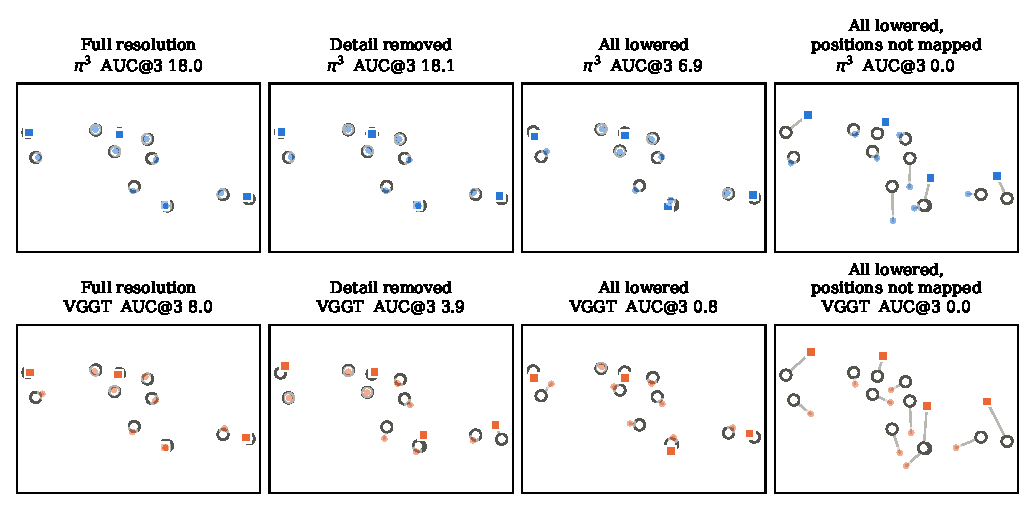
\includegraphics[width=\textwidth]{figures/fig_cameras.pdf}
  \caption{\textbf{Predicted camera layouts under the probes}, one development scene (7-Scenes \emph{Heads}, seed 42), seen from above. Open circles are the ground-truth camera centres; filled markers are the predicted ones after a similarity alignment to the ground truth, with squares for the 4 anchor views and circles for the 8 probed views; grey lines join each prediction to its ground truth. Removing fine detail leaves \pithree's layout unchanged and moves several of VGGT's cameras; lowering every stage displaces the probed views; without position mapping the layout breaks down for both models. This scene was used during development and is shown only as an illustration.}
  \label{fig:s_cameras}
\end{figure*}

\paragraph{Heads.}
The \emph{Global lowered} probe also lets the heads read the 8 views at half resolution. Letting the heads read the full-resolution tokens instead gives nearly identical results for both models (8.64 against 8.69 \auc for \pithree, 2.31 for VGGT in both cases), so the loss attributed to this probe comes from global attention rather than from the heads.

\paragraph{Encoder lowered under lowered global attention.}
When global attention is already lowered, also lowering the encoder hardly changes \pithree (8.51 against 8.46) and helps VGGT relative to removing detail (2.08 against 1.33). With global attention lowered, \pithree's accuracy is limited by that stage, and the encoder's resolution no longer matters.

\paragraph{Five scenes are not enough.}
On these 5 scenes, lowering only the keys costs \pithree almost nothing ($13.09$ against $13.17$ \auc, difference $-0.08$, interval \ci{-2.95}{2.86}), whereas on the 70 fresh scene-draws it costs 2.26 \ci{-3.58}{-0.95}. Effects of this size cannot be measured on 5 scenes, which is why the main results use the 70 draws on 7-Scenes and two further datasets.

%--------------------------------------------------------------------
\section{Hypotheses tested and rejected}
\label{sec:s_rejected}

\subsection{Shifted feature statistics}
One explanation for the cost of lowering resolution is that tokens from lower-resolution views have different statistics from full-resolution tokens, so that global attention compares mismatched features. Before each global-attention block, we measured the mean absolute difference between the per-channel means of the lowered views' tokens and those of the full-resolution views' tokens, in units of the full-resolution views' standard deviation. On the 5 development scenes it averaged 0.23 for \pithree and 0.34 for VGGT: the two groups differ by about a quarter to a third of a standard deviation. Matching the lowered views' per-channel mean and standard deviation to those of the full-resolution views before every global block made results worse, for \pithree from 5.63 to 3.48 \auc and for VGGT from 3.05 to 1.63 (\cref{tab:s_stats}). Applying the matching only to what global attention reads, without changing the tokens passed on, also made results worse. Mismatched feature statistics are thus not what costs accuracy.

\begin{table}[t]
\centering\small
\setlength{\tabcolsep}{3pt}
\begin{adjustbox}{max width=\linewidth}
\begin{tabular}{@{}lcccc@{}}
\toprule
 & \multicolumn{2}{c}{\pithree} & \multicolumn{2}{c}{VGGT} \\
\cmidrule(lr){2-3}\cmidrule(l){4-5}
All lowered, plus (5 scenes) & \auc & \aucc & \auc & \aucc \\
\midrule
nothing                                & 5.63 & 74.31 & 3.05 & 65.98 \\
statistics matched                     & 3.48 & 57.92 & 1.63 & 58.39 \\
statistics matched, read only          & 3.65 & 63.62 & 1.59 & 60.43 \\
logit bias, global attention           & 5.79 & 75.21 & 2.31 & 64.77 \\
logit bias, frame and global           & 6.83 & 77.34 & 3.40 & 68.43 \\
statistics matched + logit bias        & 3.24 & 61.43 & 2.70 & 55.57 \\
\bottomrule
\end{tabular}
\end{adjustbox}
\caption{\textbf{Corrections based on token statistics and attention mass}, on the 5 development scenes. ``Read only'' applies the matching to the tokens global attention reads but passes the original tokens on.}
\label{tab:s_stats}
\end{table}

\subsection{Attention mass}
A lowered view has about a quarter as many tokens as a full-resolution one, so it may receive too little of the softmax's attention. Adding the logarithm of the token ratio to its keys' logits gives each of its tokens the attention weight that the corresponding group of full-resolution tokens would receive if those tokens were identical. On the 5 development scenes this helped \pithree by 1.2 \auc when applied in both attention types, but on the 70 fresh scene-draws it changed \pithree by $+0.02$ \ci{-0.50}{0.53} and VGGT by $+0.78$ \ci{0.51}{1.06} (\cref{tab:s_diff}). The attention mass received by lowered views is at most a small part of the problem.

\subsection{Independent errors across input sizes}
\label{sec:s_ens}
To fuse predictions made at several input sizes, we align each prediction's cameras to a reference with a similarity transform (a rotation found by projecting the summed rotation products onto SO(3), then a least-squares scale and translation of the camera centres), average the rotations by their chordal mean and the centres arithmetically, and repeat the alignment to the fused result three times. On synthetic data with independent noise, this fusion is more accurate than every single input, as expected. \Cref{tab:s_ens} lists every combination of two and three uniform sizes on the 70 7-Scenes scene-draws. For both models, every combination is significantly worse than the best single size that costs no more compute.

\begin{table}[t]
\centering\scriptsize
\setlength{\tabcolsep}{2pt}
\begin{adjustbox}{max width=\linewidth}
\begin{tabular}{@{}lccc@{}}
\toprule
Sizes fused (tokens) & \auc & GFLOPs & vs best single at $\le$ cost \\
\midrule
\multicolumn{4}{@{}l}{\textbf{\pithree}} \\
4k+5k           & 11.16 & 17{,}912 & $-3.20$ \ci{-4.05}{-2.39} \\
4k+6k           & 10.90 & 20{,}579 & $-3.46$ \ci{-4.29}{-2.68} \\
4k+7k           & 12.15 & 22{,}774 & $-2.21$ \ci{-2.87}{-1.61} \\
5k+6k           & 12.40 & 23{,}264 & $-1.96$ \ci{-2.50}{-1.44} \\
5k+7k (fixed in advance) & 13.74 & 25{,}459 & $-0.62$ \ci{-0.99}{-0.28} \\
4k+8k           & 11.30 & 26{,}287 & $-3.06$ \ci{-3.83}{-2.33} \\
6k+7k           & 13.19 & 28{,}126 & $-1.17$ \ci{-1.49}{-0.85} \\
5k+8k           & 12.94 & 28{,}972 & $-1.42$ \ci{-1.95}{-0.91} \\
4k+5k+6k        & 11.62 & 30{,}877 & $-2.74$ \ci{-3.48}{-2.03} \\
6k+8k           & 12.33 & 31{,}639 & $-2.03$ \ci{-2.60}{-1.48} \\
4k+5k+7k        & 12.48 & 33{,}073 & $-1.88$ \ci{-2.50}{-1.29} \\
7k+8k           & 13.71 & 33{,}835 & $-0.65$ \ci{-0.94}{-0.37} \\
4k+6k+7k        & 12.25 & 35{,}740 & $-2.11$ \ci{-2.69}{-1.56} \\
4k+5k+8k        & 11.94 & 36{,}586 & $-2.42$ \ci{-3.12}{-1.76} \\
5k+6k+7k        & 13.19 & 38{,}425 & $-1.17$ \ci{-1.54}{-0.81} \\
4k+6k+8k        & 11.67 & 39{,}253 & $-2.69$ \ci{-3.38}{-2.03} \\
4k+7k+8k        & 12.60 & 41{,}448 & $-1.76$ \ci{-2.30}{-1.23} \\
5k+6k+8k        & 12.64 & 41{,}938 & $-1.72$ \ci{-2.22}{-1.23} \\
5k+7k+8k        & 13.58 & 44{,}133 & $-0.78$ \ci{-1.14}{-0.43} \\
6k+7k+8k        & 13.15 & 46{,}800 & $-1.21$ \ci{-1.59}{-0.83} \\
\midrule
\multicolumn{4}{@{}l}{\textbf{VGGT}} \\
4k+5k           & 1.63 & 21{,}909 & $-3.97$ \ci{-4.95}{-3.11} \\
5k+7k (fixed in advance) & 3.82 & 31{,}272 & $-3.31$ \ci{-4.25}{-2.51} \\
6k+8k           & 5.18 & 38{,}969 & $-1.95$ \ci{-2.55}{-1.43} \\
7k+8k           & 6.44 & 41{,}702 & $-0.69$ \ci{-0.97}{-0.43} \\
5k+7k+8k        & 4.91 & 54{,}317 & $-2.22$ \ci{-2.90}{-1.62} \\
6k+7k+8k        & 5.42 & 57{,}627 & $-1.71$ \ci{-2.25}{-1.25} \\
\bottomrule
\end{tabular}
\end{adjustbox}
\caption{\textbf{Fusing predictions from several input sizes} (7-Scenes, 70 scene-draws). Sizes are named by their token count: 4k $=224{\times}294$, 5k $=252{\times}336$, 6k $=280{\times}364$, 7k $=294{\times}392$, 8k $=322{\times}420$. The last column compares each ensemble with the most accurate single size whose compute is not higher (for \pithree always the 7k input, 14.36 \auc; for VGGT the 7k input for the cheapest ensemble and the 8k input, 7.13 \auc, for all others). For VGGT we list the cheapest ensemble, the ensemble fixed in advance and the four ensembles closest to the best single size; all 20 are significantly worse.}
\label{tab:s_ens}
\end{table}

One \pithree ensemble exceeds both of its members: 5k+8k reaches 12.94 \auc against 12.66 and 12.64, a gain of 0.28 for which we did not compute an interval. Every other ensemble lies between its members or below them.

\subsection{Aspect ratio}
Resizing frames without cropping changes their aspect ratio slightly, and differently for full- and half-resolution views (on 7-Scenes, 1.30 and 1.25 instead of 1.33). To check that this does not explain the cost of lowered resolution, we repeated the uniform, full-resolution and lowered inputs with sizes that are exactly 4:3 on 7-Scenes ($336{\times}448$ full, $168{\times}224$ half, $252{\times}336$ uniform), on the 75 scene-draws including the development scenes. The loss from lowering every stage (Full $-$ All lowered) was 7.34 \auc for \pithree with the original sizes and 7.55 with exact 4:3 sizes; for VGGT it was 5.41 and 7.71. The loss is not smaller with exact sizes, so the aspect change does not explain it. All inputs scored 1--3 \auc higher with the exact sizes, but those sizes also carry more tokens (for example 4{,}608 instead of 4{,}200 for the lowered input), so this gain cannot be attributed to the aspect ratio.

%--------------------------------------------------------------------
\section{7-Scenes precision}
\label{sec:s_floor}

\paragraph{Two-view estimates.}
For every pair of the 12 views in each of the 70 scene-draws, we detected up to 4{,}000 SIFT features per full-resolution frame, kept matches that pass Lowe's ratio test at 0.8 in both directions and are mutual nearest neighbours, and estimated an essential matrix with RANSAC (threshold 1\,px, confidence 0.9999) using an assumed pinhole camera with principal point $(320, 240)$. \Cref{tab:s_gt} compares the resulting rotations with the ground truth on the pairs with at least 100 inliers, for five assumed focal lengths; 585\,px is the value distributed with the dataset. The models' errors on the same pairs use their poses from the uniform $294{\times}392$ input.

\begin{table}[t]
\centering\small
\setlength{\tabcolsep}{3pt}
\begin{adjustbox}{max width=\linewidth}
\begin{tabular}{@{}cccccc@{}}
\toprule
Focal & Pairs & SIFT median & SIFT ${<}1^\circ$ & \pithree median & VGGT median \\
\midrule
500 & 348 & 1.86 & 6\% & 1.63 & 1.87 \\
525 & 354 & 1.86 & 6\% & 1.64 & 1.90 \\
550 & 355 & 1.90 & 6\% & 1.64 & 1.91 \\
585 & 346 & 2.04 & 4\% & 1.63 & 1.90 \\
620 & 346 & 2.21 & 3\% & 1.62 & 1.89 \\
\bottomrule
\end{tabular}
\end{adjustbox}
\caption{\textbf{Rotation error against the 7-Scenes ground truth on well-matched pairs} (degrees, 70 scene-draws). The pair set changes slightly with the assumed focal length because the inlier count does.}
\label{tab:s_gt}
\end{table}

The error of the classical estimate hardly depends on the assumed focal length, so an error in the nominal intrinsics alone does not explain it. Lens distortion, misregistration between the colour camera and the depth camera from which the poses were tracked, or errors in the tracked poses themselves would all produce a floor of this kind; we did not determine which.

\paragraph{Refining the models' poses with two-view geometry.}
We also used the classical estimates to refine each model's predicted poses. A pair estimate is accepted if it has at least 30 inliers and its rotation is within 15\textdegree{} of the model's; accepted pairs replace the model's relative rotation and translation direction, and all pairs are fused back into one set of poses by rotation averaging and a least-squares solve for the camera centres, in which accepted pairs constrain only the direction between two cameras and keep the model's distance. With no accepted pair, the output equals the model's poses. These thresholds were fixed before any real image was processed. Only 28\% of pairs were accepted. \Cref{tab:s_geo} shows that refinement lowers \pithree's \auc at every input size and its \aucc by 2.0 to 3.4, while it raises VGGT's \auc at the three smallest sizes, where VGGT is far from its preferred size. A classical estimate is thus not more accurate than \pithree against this ground truth.

\begin{table}[t]
\centering\small
\setlength{\tabcolsep}{2.5pt}
\begin{adjustbox}{max width=\linewidth}
\begin{tabular}{@{}lcccc@{}}
\toprule
 & \multicolumn{2}{c}{\pithree \auc} & \multicolumn{2}{c}{VGGT \auc} \\
\cmidrule(lr){2-3}\cmidrule(l){4-5}
Uniform input & model & refined (difference) & model & refined (difference) \\
\midrule
$224{\times}294$ & 9.36 & 7.88 \ci{-2.25}{-0.74} & 1.10 & 2.39 \ci{0.90}{1.72} \\
$252{\times}336$ & 12.66 & 9.88 \ci{-3.72}{-1.88} & 2.42 & 3.69 \ci{0.74}{1.80} \\
$280{\times}364$ & 11.70 & 9.39 \ci{-3.13}{-1.49} & 3.71 & 4.46 \ci{0.22}{1.28} \\
$294{\times}392$ & 14.36 & 10.91 \ci{-4.40}{-2.54} & 5.61 & 5.92 \ci{-0.32}{0.93} \\
$322{\times}420$ & 12.64 & 9.80 \ci{-3.67}{-2.02} & 7.13 & 6.71 \ci{-1.09}{0.24} \\
\bottomrule
\end{tabular}
\end{adjustbox}
\caption{\textbf{Refining predicted poses with classical two-view geometry} (7-Scenes, 70 scene-draws). Intervals are for the difference between refined and model poses.}
\label{tab:s_geo}
\end{table}

%--------------------------------------------------------------------
\section{How the study developed}
\label{sec:s_history}

This study began as an attempt to design a training-free change to these models that would let them process some views at lower resolution without losing accuracy. We report how it developed because it explains the probes and because several of our pre-stated tests failed.

Our first design fed the lowered views to the encoder upsampled to full size, ran frame attention at full resolution, and let global attention read them at half resolution; this is the \emph{Global lowered, detail removed} probe of \cref{tab:s_7s}. On the 5 development scenes, it was better than lowering every stage for \pithree (8.40 against 5.63 \auc, \cref{tab:s_dev}) and worse for VGGT (1.33 against 3.05). We then wrote down, before running them, a sequence of tests, each with a numeric pass rule:
\begin{itemize}[nosep,leftmargin=*]
  \item \textbf{Zero-cost corrections} (\cref{tab:s_stats}): pass if the best correction improved the lowered input by at least 2 \auc and in at least 4 of 5 scenes. It failed for both models (best: $+1.20$ for \pithree, $+0.35$ for VGGT).
  \item \textbf{Real pixels with global attention lowered}: pass if it beat a uniform input of the same nominal budget by at least 2 \auc in at least 4 of 5 scenes. It failed for \pithree ($+1.21$, 2 of 5 scenes) and passed for VGGT ($+2.13$, 5 of 5), but on the 70 fresh scene-draws VGGT's \emph{Global lowered} input (3.28) is below the uniform $280{\times}364$ input of similar compute (3.71), so we did not pursue it.
  \item \textbf{Encoder lowered, with and without keys lowered}, on the 70 fresh draws: pass if within 1 \auc of the \emph{Detail removed} input, significantly better than a uniform input of no lower compute, and at most 2 \aucc below the smallest uniform input. Both failed for both models (\cref{tab:s_7s,tab:s_diff}).
  \item \textbf{Fusing predictions across sizes}: pass if the fixed pair 5k+7k beat the best single size at no more compute with an interval above zero. It failed for both models (\cref{tab:s_ens}).
  \item \textbf{Refining poses with two-view geometry}: pass if the smallest input plus refinement beat the best single input. It failed for both models (\cref{tab:s_geo}).
\end{itemize}
Each failure removed one explanation of where the models use resolution, and together they led to the probing study in the main paper. All results above, including the failed tests, use the same code, data and metric as the main paper.

%--------------------------------------------------------------------
\section{Reproducing the results}
\label{sec:s_repro}

The code accompanying this paper contains the stage decomposition and probes, the identity check, the data preparation for all three datasets, the configuration file of every probe, and the scripts that produce each table here from the stored per-scene results. Every result file records the code version, the configuration, the frames used with their checksums, the checkpoint and its checksum, and the GPU, and the runner refuses to overwrite a result produced under a different configuration. A full run of all experiments in this paper takes several hours on one RTX 5090.

\end{document}
